\section{Formal systems}

\begin{notion}

A \textbf{formal system} is a system of symbols and rules governing their
manipulation.

\end{notion}

A formal system is a purely mental construct. To be used to any effect in the
real world, a formal system must be realised by a physical system.

\begin{notion}

A \textbf{physical system} is a system of physical symbols and processes
manipulating them. 

\end{notion}

For instance, this document was typeset by a physical system. The symbols in
question are typographical symbols, and the process of typesetting is the
typographical composition of such symbols.

Out of consideration for the reader, the formal systems presented herein, deal
in the same typographical symbols, and govern their typographical composition
in this document.

The reader, equipped with a writing instrument, is another physical system. The
reader is invited to realise the formal systems in question at their leisure,
in attempt to discredit the physical realisations herein.

\section{Basic definitions and notation}

We begin by introducing some notation for sets, objects, and judgements,
leading to a definition of a formal system, as regarded in this document. The
matters of notation address the typesetting of this document, and bear no
logical significance otherwise.

\subsection{Sets}

\begin{definition}

A \textbf{set} is a collection of distinct \textbf{elements}.

\end{definition}

The notions of ``collection'' and ``distinct'' arise from our choice of
notation.

\begin{notation}

Two typographical symbols are \textbf{distinct}, if the reader can at a glance
tell a difference between them.

\end{notation}

\begin{notation}

The \textbf{elements} of a set are denoted by distinct typographical symbols,
which fit inside the following box:

\begin{center}
\framebox{\vbox to 12pt {\vfil \hbox to 48pt {} \vfil}}
\end{center}

\end{notation}

If the elements of a set can be denoted by distinct typographical symbols, the
set can be denoted elementarily by denoting the elements in a sequence. 

\begin{notation}

A set is \textbf{denoted elementarily} by denoting the elements in a
typographical sequence, separated by commas($,$), and enclosed in
braces($\set{}$).

\end{notation}

For instance, $\set{\symb{a},\symb{b},\symb{c}}$ elementarily denotes exactly
the collection of elements $\symb{a}$, $\symb{b}$, and $\symb{c}$.  This
notational convention superimposes an order on the elements in a set. This
order bears no logical significance.

\begin{notational-corollary}

The elements of a set, when denoted elementarily in a different order, do not
denote a distinguished set.

\end{notational-corollary}

This notation is useful as it permits the reader to confirm that the elements
are distinct by considering the elements in sequence, and confirming, for each
symbol, that it does not appear more than once in the sequence. That is,
provided that the set is finite.

\begin{notion}

A set is \textbf{finite} if it can eventually be denoted elementarily.

\end{notion}

This notation does not permit the denotation of an infinite set, and is fairly
impractical for denoting large finite sets. To that end, the reader will be
presented with a procedure by which the elements of the set could be denoted
elementarily, had we the typographical tools and the (possibly infinite) time
to do so. When reasoning about sets denoted by such a ``generating procedure'',
we will reason about the procedure rather than elements themselves.

\subsection{Objects}

\begin{definition}

An \textbf{alphabet} is a finite set.

\end{definition}

\begin{definition}

An \textbf{object} is either an element drawn from an alphabet, or a collection
of objects, put in relation.

\end{definition}

\begin{notation}

An object is denoted as a typographical composition of the objects in question,
which fits inside the following box:

\begin{center}
\framebox{\vbox to 48pt {\vfil \hbox to 48pt {} \vfil }}
\end{center}

\end{notation}

For instance, given the alphabet $\set{a,b,c}$, we may consider, among
others, the following objects:

\begin{center}
$abc$
\quad\quad\quad
$\begin{matrix}
  & a &   \\
a & a & a \\
  & a &
\end{matrix}$
\quad\quad\quad
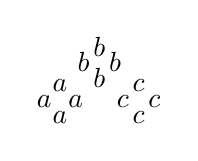
\begin{tikzpicture}
\draw (-0.5,0.0) node {$a$};
\draw (-0.7,0.2) node {$a$};
\draw (-0.3,0.2) node {$a$};
\draw (-0.5,0.4) node {$a$};
\draw (0.0,0.9) node {$b$};
\draw (0.2,0.7) node {$b$};
\draw (-0.2,0.7) node {$b$};
\draw (0.0,0.5) node {$b$};
\draw (0.5,0.0) node {$c$};
\draw (0.7,0.2) node {$c$};
\draw (0.3,0.2) node {$c$};
\draw (0.5,0.4) node {$c$};
\end{tikzpicture}

\end{center}

\begin{definition}

An object is \textbf{empty} if it is neither an element of the alphabet, nor a
collection of any objects.

\end{definition}

\begin{notation}

For alphabets not containing the element $\varepsilon$, we denote the empty
object by $\varepsilon$, out of considerations for readability.

\end{notation}

\subsection{Variables}

\begin{definition}

A \textbf{variable} is an object which is a placeholder for another object.

\end{definition}

\begin{definition}

A variable occurring multiple times in an object, is a placeholder for the same
object.

\end{definition}

\begin{definition}

An object is \textbf{concrete} if it is not a variable.

\end{definition}

\begin{definition}

A variable is \textbf{bound} if it is a placeholder for a particular object,
and \textbf{free} otherwise.

\end{definition}

\begin{notation}

When we say ``an object $O$'', we really mean ``a variable $O$, bound to a
particular object''.

\end{notation}

\begin{definition}

An variable is \textbf{fresh} for an object $O$, if it does not occur in $O$.

\end{definition}

%\begin{definition}

%We say that an object $O$ is ``alpha-equivalent'' to an object $O'$, denoted
%$O=_{\alpha}O'$, if we can construct $P$ from $O$ by replacing variables in $O$
%with fresh

%\end{definition}

\subsection{Judgements}

\begin{definition}

A \textbf{judgement} is an object.

\end{definition}

Judgements come in various forms, putting objects in various relations. For
instance, given the objects \symb{0}, \symb{1}, $\text{nat}$, $=$, and $+$, we
may consider, among others, the following judgements:

\begin{table}[h!]
\centering
\begin{tabular}{|l|l|}
\hline
\textbf{Judgement} & \textbf{Reading} \\
\hline
$\symb{0}\;\text{nat}$ & \symb{0} is a natural number. \\
\hline
$\symb{1}=\symb{0}+\symb{1}$ & \symb{1} is the sum of \symb{0} and \symb{1}.\\
\hline
\end{tabular}
\end{table}

\begin{definition}

An \textbf{inference rule} is a collection of judgements called the
\textbf{premises} and a judgement called the \textbf{conlusion} of the
inference rule.

\end{definition}

\begin{notation}

An inference rule is denoted by denoting the premises in a typographical
sequence, separated by due whitespace, over a denotation of the conclusion. The
premises and conclusion are separated by a horizontal bar.

\end{notation}

For instance, for a variable $n$, we may consider an inference rule with the
single premise $n\;\text{nat}$, and the conclusion $\symb{s}(n)\;\text{nat}$:

$$
\judgement[Nat-Rec]{
  n\;\text{nat}
}{
  \symb{s}(n)\;\text{nat}
}
$$

This rule reads: if $n$ is a natural number, then its successor is also a
natural number.

\begin{definition}

An \textbf{axiom} is an inference rule with no premises.

\end{definition}

For instance, we may consider an axiom with the conclusion
$\symb{z}\;\text{nat}$:

$$
\judgement[Nat-Z]{
}{
  \symb{z}\;\text{nat}
}
$$

This rule reads: zero is a natural number.

\begin{definition}

A judgement $J_0$ is \textbf{structurally subsumed} by a judgement $J_1$,
denoted $J_0\subseteq J_1$, if $J_1$ can be constructed from $J_0$ by replacing
objects in $J_0$ by variables.

\end{definition}

For instance, $\symb{s}(n)\;\text{nat}\subseteq n\;\text{nat}$.

\begin{remark}

There is no relation between the variables on the left- and right-hand side of
$\subseteq$.

\end{remark}

\begin{definition}

A \textbf{judgement form} is a judgement $J$, defined by a collection of
inference rules having a conclusion structurally subsumed by $J$.

\end{definition}

\begin{notation}

A judgement form is denoted by denoting the judgement in a box.

\end{notation}

For instance, we may consider the judgement form \fbox{$n\;\text{nat}$},
defined by the rules \ruleref{Nat-Rec} and \ruleref{Nat-Z}, which reads: $n$ is
a natural number. This reading is not incidental, and indicates that
\fbox{$n\;\text{nat}$} specifies a procedure for elementarily denoting the
elements of the set of natural numbers.

\subsection{Derivations}

% TODO: unification

%\begin{definition}

%A judgement is \textbf{derivable} either if it unifies with a conclusion of an
%inference rules whose premises are derivable.

%\end{definition}

% TODO: derivations and their notation

%\begin{definition}

%To show that a judgement is derivable, we present a \textbf{derivation} of that
%judgement.

%\end{definition}

TODO: definitions

A judgement form that deals in a single object, specifies a set of objects,
indeed the objects occurring in all derivable judgements of that form. A
judgement form can therefore be used to specify a procedure by which the
elements of a set can be denoted elementarily.

% TODO: actually define the order in which this is done, probably have to
% introduce derivations.

For instance, here are the first couple of natural numbers by the judgement
form \fbox{$n\;\text{nat}$}:

$$\set{\symb{z}, \symb{s}(\symb{z}), \symb{s}(\symb{s}(\symb{z})),
\symb{s}(\symb{s}(\symb{s}(\symb{z}))),
\symb{s}(\symb{s}(\symb{s}(\symb{s}(\symb{z})))),
\symb{s}(\symb{s}(\symb{s}(\symb{s}(\symb{s}(\symb{z}))))), \ldots }$$

\subsection{Syntax}

Using judgements to syntactically define a set of objects is unconventional.

\subsubsection{Backus-Naur Form}

\subsubsection{Signatures}

\subsection{Functions}

%\begin{definition}

%A \textbf{function} is a judgement form that puts in relation zero or more
%\textbf{input} variables, and an \textbf{output} variable.

%\end{definition}

%\begin{notation}

%A function 

%\end{notation}

% An enumerable set is any set that denotes the set of natural numbers.
